\section{变量分块与交替优化}
\label{sec:opt-sto-block}

前面几节都在节省读取：每步读得少，但更新全部坐标。本节转到图~\ref{fig:opt-sto-sum-vs-block}的右半边，每轮只改变一部分变量。这样做的理由有两种：一部分变量的子问题可能便宜得多，甚至有闭式解；或者变量本身分成性质不同的几组，例如矩阵分解中的两个因子。问题在于，各块分别得到的改善能否拼成整体的改善，以及变量之间的耦合会留下什么困难。

\subsection{块梯度与块邻近更新}
\label{sec:opt-sto-block-gradient}

\paragraph{块光滑常数}
把坐标$\{1,\dots,d\}$划分为互不相交的块$J_1,\dots,J_B$，记$\bm x_J$为$\bm x$在块$J$上的分量，$\nabla_Jf(\bm x)$为对应的偏梯度，$\bm U_J\bm h$表示把$\bm h\in\mathbb R^{|J|}$放回块$J$、其余坐标补零的向量。若只沿块$J$移动时梯度的变化满足
\[
  \lVert\nabla_Jf(\bm x+\bm U_J\bm h)-\nabla_Jf(\bm x)\rVert_2\leq L_J\lVert\bm h\rVert_2\quad\text{对一切}\ \bm x,\bm h,
\]
就称$f$关于块$J$是$L_J$光滑的。与下降引理的证明完全相同，沿块$J$有二次上界$f(\bm x+\bm U_J\bm h)\leq f(\bm x)+\langle\nabla_Jf(\bm x),\bm h\rangle+\tfrac{L_J}2\lVert\bm h\rVert_2^2$。取$\bm h=-\nabla_Jf(\bm x)/L_J$，目标至少下降$\lVert\nabla_Jf(\bm x)\rVert_2^2/(2L_J)$。块光滑常数不超过整体的$L$，常常小得多：对最小二乘，单个坐标$j$的常数是$L_j=\lVert\bm A_{:,j}\rVert_2^2/n+\lambda$，即一个对角元，而$L$是整个矩阵的最大特征值。

\paragraph{计算单位}
一次块更新与一次完整循环是不同的计算单位。以最小二乘的单坐标更新为例，若维护残差$\bm r=\bm A\bm x-\bm b$，则$\partial_jf(\bm x)=\bm A_{:,j}^\top\bm r/n+\lambda x_j$只需$O(n)$，更新$x_j$后残差改变$\bm A_{:,j}\Delta x_j$，也是$O(n)$。遍历全部$d$个坐标一次的代价约为$O(nd)$，与一次梯度下降相当。因此比较坐标方法与梯度方法时，应以完整循环或总计算量为单位，而不是比较单步。

\paragraph{块邻近更新}
目标带有按块可分的非光滑项$F(\bm x)=f(\bm x)+\sum_kr_k(\bm x_{J_k})$时，把块梯度步换成块邻近梯度步：
\[
  \bm x_J\gets\operatorname{prox}_{r_J/L_J}\Bigl(\bm x_J-\frac1{L_J}\nabla_Jf(\bm x)\Bigr),
\]
其余块不变。它是第~\ref{chap:opt-nonsmooth}章邻近梯度法在单块上的版本。那里对凸的非光滑项、步长取光滑常数的倒数时证明了复合目标不增；把光滑常数换成块常数$L_J$，同一论证在单块上照样成立。$r_k=\lambda_1|\cdot|$的单坐标情形就是对最小二乘做软阈值，这是求解套索问题的常用方法。可分性在这里是本质的：非光滑项必须按块拆开，每块的邻近映射才能单独计算。

\paragraph{选块规则与新值的读取}
选块有三种常见规则。\emph{循环}规则按固定顺序依次更新，每块更新后立即用新值计算下一块的偏梯度。\emph{随机}规则每轮独立地均匀抽一块。\emph{贪心}规则选偏梯度最大的一块，需要维护全部偏梯度。另有一种并行做法让所有块都用上一轮的旧值同时更新，这实际上是一次带特殊步长的全梯度步，块上界不能保证它下降。对随机规则，每块的二次上界可以直接取期望。

\begin{theorem}[随机块坐标下降]
\label{thm:opt-sto-random-block}
设$f$关于每个块$J_k$是$L_{J_k}$光滑的，记$L_{\mathrm b}=\max_kL_{J_k}$，有下界$f^\star$。每轮与历史独立地均匀抽取一块$J$，令$\bm x_J\gets\bm x_J-\nabla_Jf(\bm x)/L_J$。则
\[
  \mathbb E_tf(\bm x^{(t+1)})\leq f(\bm x^{(t)})-\frac1{2B}\sum_{k=1}^B\frac{\lVert\nabla_{J_k}f(\bm x^{(t)})\rVert_2^2}{L_{J_k}}\leq f(\bm x^{(t)})-\frac{\lVert\nabla f(\bm x^{(t)})\rVert_2^2}{2BL_{\mathrm b}} .
\]
若$f$还是$\mu$强凸的，则$\mathbb Ef(\bm x^{(t)})-f^\star\leq\bigl(1-\mu/(BL_{\mathrm b})\bigr)^t\bigl(f(\bm x^{(0)})-f^\star\bigr)$。
\end{theorem}

\begin{proof}
抽到块$J_k$的概率为$1/B$，此时目标至少下降$\lVert\nabla_{J_k}f\rVert_2^2/(2L_{J_k})$，取平均即得第一个不等式；再用$L_{J_k}\leq L_{\mathrm b}$与$\sum_k\lVert\nabla_{J_k}f\rVert_2^2=\lVert\nabla f\rVert_2^2$。强凸时，对强凸下界$f(\bm y)\geq f(\bm x)+\langle\nabla f(\bm x),\bm y-\bm x\rangle+\tfrac\mu2\lVert\bm y-\bm x\rVert_2^2$两边对$\bm y$取最小值，得$f^\star\geq f(\bm x)-\lVert\nabla f(\bm x)\rVert_2^2/(2\mu)$，即$\lVert\nabla f(\bm x)\rVert_2^2\geq2\mu(f(\bm x)-f^\star)$。代入后减去$f^\star$、取全期望并反复使用即可。
\end{proof}

这个速率与随机抽样的随机梯度不同：读数没有噪声，只是每轮只走一个方向，所以收敛是线性的\scite{nesterov2012efficiency}。$B$次块更新大约等于一次完整循环，其收缩约为$(1-\mu/(BL_{\mathrm b}))^B\approx1-\mu/L_{\mathrm b}$；与梯度下降每步的$1-\mu/L$相比，块常数$L_{\mathrm b}$越小于$L$，坐标方法的优势越大。

\paragraph{阶梯路径与耦合}
图~\ref{fig:opt-sto-coordinate-descent}(a)在二次目标$\Phi(u,v)=\tfrac12(u-v)^2+\tfrac12(u-1)^2$上画出逐块精确最小化的循环坐标下降：路径只能沿坐标轴走，形成阶梯，在等高线细长且倾斜的方向上，每一阶都很短。精确地，固定$v$时最优$u=(v+1)/2$，固定$u$时最优$v=u$，所以每轮$v^{(t+1)}-1=\tfrac12(v^{(t)}-1)$，误差逐轮减半。变量间的耦合越强（等高线越斜越扁），阶梯越密，收敛越慢。

\begin{figure*}[!htbp]
  \centering
  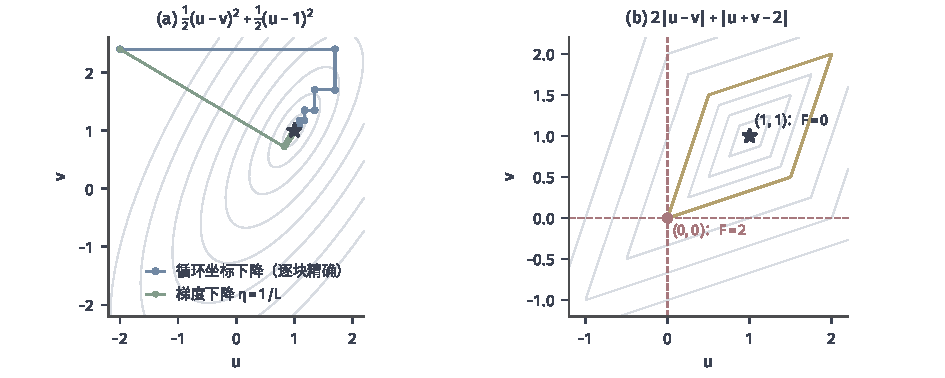
\includegraphics[width=160mm]{figures/03-optimization-evolution-and-signals/01-optimization/matplotlib/c6-coordinate-descent/figure.pdf}
  \caption{坐标下降的阶梯路径与停滞。(a) $\Phi(u,v)=\tfrac12(u-v)^2+\tfrac12(u-1)^2$，从$(-2,2.4)$出发：蓝线为循环坐标下降，每次精确最小化一个变量，$v$的误差逐轮减半；绿线为步长$1/L$的梯度下降。(b) 凸而不可分的非光滑目标$F(u,v)=2|u-v|+|u+v-2|$：在原点沿两条红色虚线方向，$F$都在原点取到唯一最小值$2$，坐标下降从原点出发永远不动；黄色为水平集$F=2$，真正的最小点是$(1,1)$，$F=0$。}
  \label{fig:opt-sto-coordinate-descent}
\end{figure*}

\paragraph{耦合约束与不可分非光滑项}
块方法的两类失败都来自耦合。第一类是约束把块绑在一起。若可行域是$\sum_jx_j=1$，从可行点出发只改一个坐标就会离开可行域，单坐标步要么不动、要么不可行；必须一次更新至少两个坐标，并让它们的变化相互抵消。第二类是非光滑项不可分。图~\ref{fig:opt-sto-coordinate-descent}(b)中$F(u,v)=2|u-v|+|u+v-2|$是凸函数，在原点$F=2$。固定$v=0$，$F(u,0)=2|u|+|u-2|$在$u<0$时斜率为$-3$，在$0<u<2$时斜率为$1$，所以$u=0$是唯一最小点；固定$u=0$同理。原点因此是每个坐标方向上的严格最小点，坐标下降在此永远停住，而$F(1,1)=0$。光滑时不会发生这种情况：各块偏梯度都为零就意味着整个梯度为零。

下降结论必须与实际规则匹配：循环、随机与贪心规则的保证各不相同，并行更新需要另外的步长条件；子问题若只近似求解，块上的下降量要扣除子问题误差，第~\ref{sec:opt-sto-perturbation}节会统一讨论这类误差。

\subsection{交替最小化}
\label{sec:opt-sto-alternating}

\paragraph{逐块求解条件子问题}
当某一块的子问题可以精确或高精度求解时，不必只走一步梯度，可以直接求出固定其余块后的最优解。对两块变量的目标$\Phi(\bm u,\bm v)$，\term{交替最小化}（alternating minimization）依次执行
\[
  \bm u^{(t+1)}\in\argmin_{\bm u}\Phi(\bm u,\bm v^{(t)}),\qquad
  \bm v^{(t+1)}\in\argmin_{\bm v}\Phi(\bm u^{(t+1)},\bm v).
\]
两步分别不增，连起来就是一轮改善：
\[
  \Phi(\bm u^{(t+1)},\bm v^{(t+1)})\leq\Phi(\bm u^{(t+1)},\bm v^{(t)})\leq\Phi(\bm u^{(t)},\bm v^{(t)}).
\]
条件子问题的最小点可能不唯一，这时算法必须事先规定\emph{平局规则}，例如“若当前值已是最小点之一就保持不变”，否则迭代序列没有明确定义。若子问题只近似求解，只要每块的返回值不比当前值差，单调性仍然成立；更细的精度要求留到误差分析。

\paragraph{分别凸不等于联合凸}
交替最小化常用于“固定一块后是凸问题”的目标，例如矩阵分解$\lVert\bm Y-\bm U\bm V^\top\rVert_F^2$：固定$\bm V$是关于$\bm U$的最小二乘，反之亦然。但分别凸并不保证联合凸，逐块精确也不保证达到全局最优。最小的例子是$\Phi(u,v)=\tfrac12(uv-1)^2$，它对$u$、对$v$分别是凸二次函数。从$(0,0)$出发，固定$v=0$时$\Phi(u,0)=\tfrac12$与$u$无关，每个$u$都是最小点，按“保持不变”的平局规则停在$u=0$；固定$u=0$同理。算法停在目标值$\tfrac12$，而全局最小值是$0$，在双曲线$uv=1$上取得。

加入正则项能消除平局，却消除不了停滞。$\Phi_\rho(u,v)=\tfrac12(uv-1)^2+\tfrac\rho2(u^2+v^2)$，$0<\rho<1$，条件子问题有唯一解$u=v/(v^2+\rho)$与$v=u/(u^2+\rho)$。从$(0,0)$出发，两式都给出$0$，算法仍停在原点；原点是驻点，其Hessian$\begin{bmatrix}\rho&-1\\-1&\rho\end{bmatrix}$有负特征值$\rho-1$，是一个鞍点。图~\ref{fig:opt-sto-alternating}取$\rho=0.05$：从$(3,0.1)$出发，路径沿弯曲的谷底以阶梯形逼近最小点$u=v=\sqrt{1-\rho}\approx0.975$，目标值从约$0.470$降到$8$轮后的约$0.0499$，最小值是$\rho-\rho^2/2=0.04875$；越靠近谷底，每一阶越短，这正是耦合造成的慢收敛；从原点出发则一步也不动，目标值停在$0.5$。

\begin{figure}[!htbp]
  \centering
  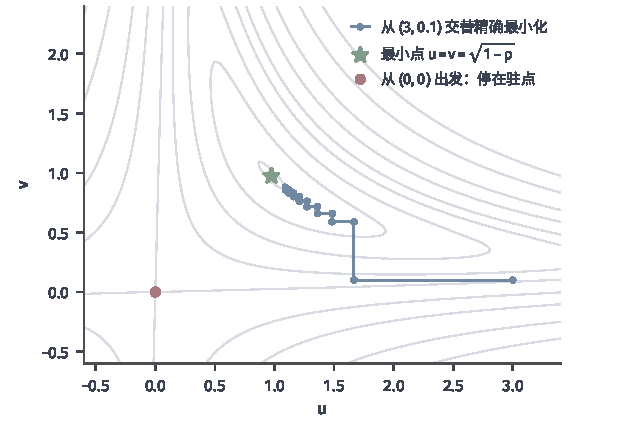
\includegraphics[width=105mm]{figures/03-optimization-evolution-and-signals/01-optimization/matplotlib/c6-alternating/figure.pdf}
  \caption{双线性目标上的交替最小化。$\Phi_\rho(u,v)=\tfrac12(uv-1)^2+\tfrac\rho2(u^2+v^2)$，$\rho=0.05$，灰色为等高线。蓝色阶梯从$(3,0.1)$出发，交替取$u=v/(v^2+\rho)$与$v=u/(u^2+\rho)$，画出前$8$轮，逐步逼近绿色星号处的最小点$u=v=\sqrt{1-\rho}$（另一最小点$u=v=-\sqrt{1-\rho}$未画出）。红点为原点：两个条件子问题的唯一解都是$0$，迭代停在这个鞍点。}
  \label{fig:opt-sto-alternating}
\end{figure}

\paragraph{能保证什么}
交替最小化的结论需要分层陈述。第一层是目标值单调不增，只要求每块返回不比当前更差的点；目标有下界时目标值序列收敛，但这并不说明迭代点收敛。第二层是聚点的块最优性：在目标连续、各条件子问题有唯一解等条件下，迭代序列的聚点在每一块上都是条件最优的；若目标还连续可微且无约束，各块偏梯度为零合起来就是整体驻点。图~\ref{fig:opt-sto-coordinate-descent}(b)说明非光滑不可分时这一步会失败。第三层是全局最优：联合凸时驻点就是全局最小点；不联合凸时，如上面的原点所示，驻点可能是鞍点。第四层是整个序列收敛到一点，这需要更强的条件，例如强凸性。期望最大化算法等具体统计方法也具有“交替求解条件子问题”的结构，在相应的概率模型建立之后，会复用这里的单调性论证，并同样面对停在非全局点的问题。
